\documentclass[11pt]{standalone}
\usepackage{tikz}
\begin{document}

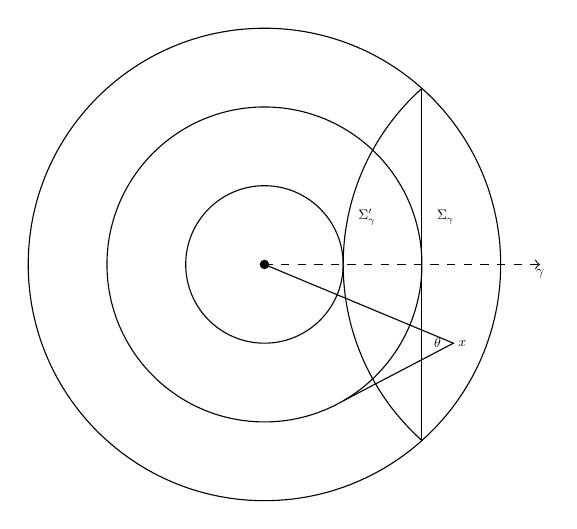
\begin{tikzpicture}[every node/.style={scale=.5}]
  \draw[fill] (0,0) circle [radius=1.5pt];
  \draw (0,0) circle [radius=1cm];
  \draw (0,0) circle [radius=2cm];
  \draw (0,0) circle [radius=3cm];
  \draw [->,dashed] (0,0)--(3.5,0) node [below]{$\gamma$};
  {
    \clip (0,0) circle [radius=3cm];
    \draw (4,0) circle [radius=3cm];
    \draw (2,-3)--(2,3);
  }
  \draw (0,0)--(2.4,-1) node[right] {$x$}--(1,{-sqrt(3)});
  \node at (2.2,-1) {$\theta$};
  \node at (1.3, 0.6) {$\Sigma_{\gamma}'$};
  \node at (2.3, 0.6) {$\Sigma_{\gamma}$};
\end{tikzpicture}


\end{document}
